\documentclass[tikz,border=10pt]{standalone}
\usetikzlibrary{angles, quotes, calc, positioning, shapes.geometric, shapes.misc, decorations.markings}

\begin{document}

% Q1
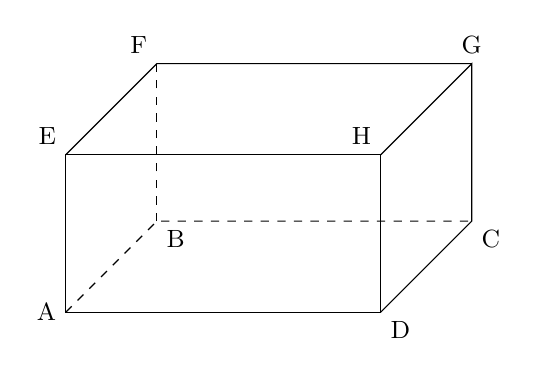
\begin{tikzpicture}[scale=1, transform shape]
    % Define the points of the cube
    \coordinate (A) at (0,0,0);
    \coordinate (B) at (0,0,-3);
    \coordinate (C) at (4,0,-3);
    \coordinate (D) at (4,0,0);
    \coordinate (E) at (0,2,0);
    \coordinate (F) at (0,2,-3);
    \coordinate (G) at (4,2,-3);
    \coordinate (H) at (4,2,0);

    % Draw the visible edges of the cube
    \draw (A) -- (D) -- (H) -- (E) -- cycle; % bottom face
    \draw (D) -- (C) -- (G) -- (H); % right face
    \draw (E) -- (F) -- (G); % top face

    % Draw the hidden edges of the cube
    \draw[dashed] (A) -- (B) -- (C);
    \draw[dashed] (B) -- (F);

    % Place the labels with smaller font size
    \node at (A) [left,font=\small] {A};
    \node at (B) [below right,font=\small] {B};
    \node at (C) [below right,font=\small] {C};
    \node at (D) [below right,font=\small] {D};
    \node at (E) [above left,font=\small] {E};
    \node at (F) [above left,font=\small] {F};
    \node at (G) [above,font=\small] {G};
    \node at (H) [above left, font=\small] {H};
    
\end{tikzpicture}

% Q2
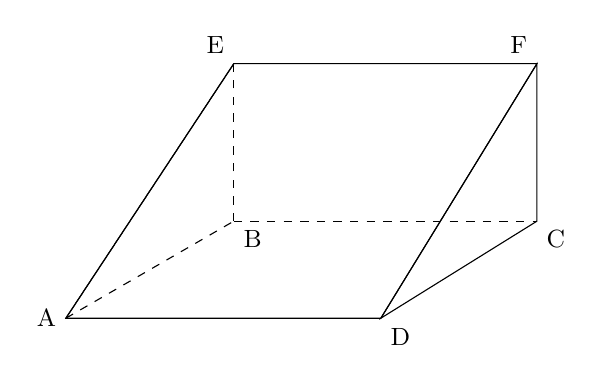
\begin{tikzpicture}[scale=1, transform shape]
    % Define the points of the cube
    \coordinate (A) at (0,0.5,0);
    \coordinate (B) at (0.4,0,-4.5);
    \coordinate (C) at (4.25,0,-4.5);
    \coordinate (D) at (4,0.5,0);
    \coordinate (E) at (0.4,2,-4.5);
    \coordinate (F) at (4.25,2,-4.5);

    % Draw the visible edges of the cube
    \draw (A) -- (E) -- (F) -- (D) -- cycle;
    \draw (D) -- (F) -- (C) -- cycle;
    \draw (A) -- (E);
    \draw[dashed] (A) -- (B);
    \draw[dashed] (B) -- (E);
    \draw[dashed] (B) -- (C);

    % Place the labels with smaller font size
    \node at (A) [left,font=\small] {A};
    \node at (B) [below right,font=\small] {B};
    \node at (C) [below right,font=\small] {C};
    \node at (D) [below right,font=\small] {D};
    \node at (E) [above left,font=\small] {E};
    \node at (F) [above left,font=\small] {F};
    
\end{tikzpicture}

% Q3
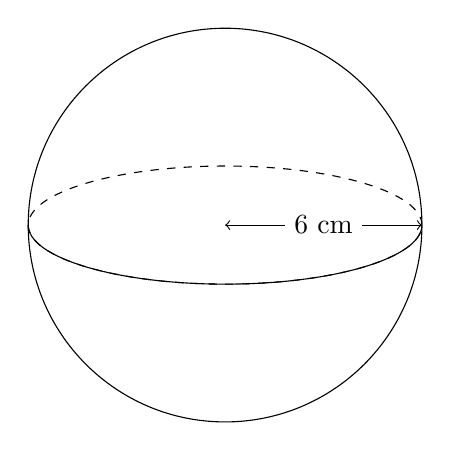
\begin{tikzpicture}
    % Define the radius for the circle
    \def\radius{2.5}
    \def\eccentricity{.3} % Eccentricity of the ellipse

    % Draw the main circle representing the sphere
    \draw (0,0) circle[radius=\radius];

    % Draw the solid bottom half of the ellipse from A to B
    \draw (-\radius,0) arc[start angle=180, end angle=360, x radius=\radius, y radius=\radius*\eccentricity];

     \draw[dashed] (-\radius,0) arc[start angle=-180, end angle=360, x radius=\radius, y radius=\radius*\eccentricity];

    % Draw the diameter line with label
    \draw[<->] (0,0) -- (\radius,0) node[midway, fill=white] {$6$ cm};
    
\end{tikzpicture}

% Q4
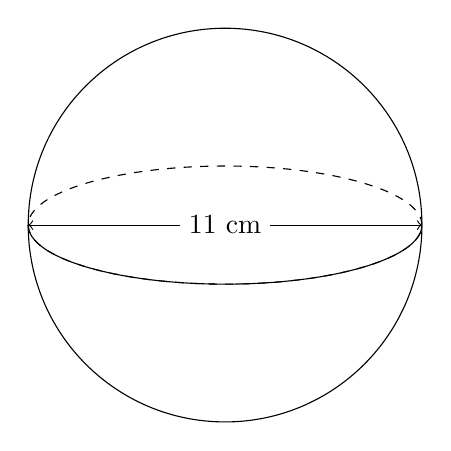
\begin{tikzpicture}
    % Define the radius for the circle
    \def\radius{2.5}
    \def\eccentricity{.3} % Eccentricity of the ellipse

    % Draw the main circle representing the sphere
    \draw (0,0) circle[radius=\radius];

    % Draw the solid bottom half of the ellipse
    \draw (-\radius,0) arc[start angle=180, end angle=360, x radius=\radius, y radius=\radius*\eccentricity];

    % Draw the dashed top half of the ellipse
     \draw[dashed] (-\radius,0) arc[start angle=-180, end angle=360, x radius=\radius, y radius=\radius*\eccentricity];

    % Draw the diameter line with label
    \draw[<->] (-\radius,0) -- (\radius,0) node[midway, fill=white] {$11$ cm};
    
\end{tikzpicture}

% Q5
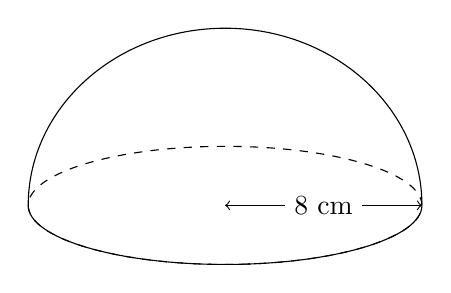
\begin{tikzpicture}
    % Define the radius for the circle
    \def\radius{2.5}
    \def\eccentricity{.3} % Eccentricity of the ellipse

    % Draw the solid bottom half of the ellipse
    \draw (-\radius,0) arc[start angle=180, end angle=360, x radius=\radius, y radius=\radius*\eccentricity];

    % Draw the dashed top half of the ellipse
     \draw[dashed] (-\radius,0) arc[start angle=-180, end angle=360, x radius=\radius, y radius=\radius*\eccentricity];

     \draw (\radius,0) arc[start angle=0, end angle=180, x radius=\radius, y radius=\radius*\eccentricity*3];

    % Draw the diameter line with label
    \draw[<->] (0,0) -- (\radius,0) node[midway, fill=white] {$8$ cm};
    
\end{tikzpicture}

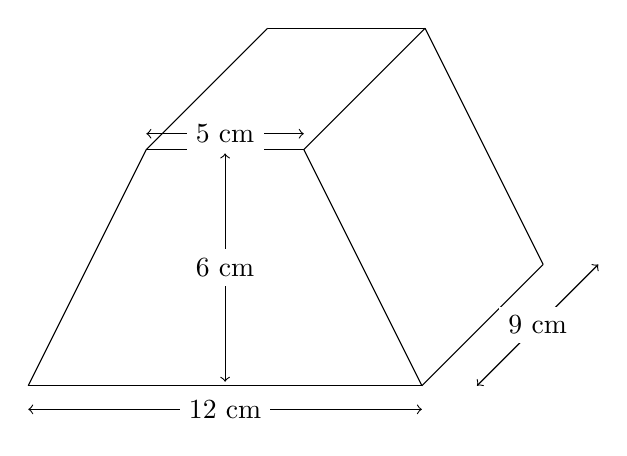
\begin{tikzpicture}[scale=1, transform shape]
    % Define the points of the cube
    \coordinate (A) at (0,0,0);
    \coordinate (B) at (5,0,0);
    \coordinate (C) at (1.5,3,0);
    \coordinate (D) at (3.5,3,0);

    \coordinate (E) at (0,0,-4);
    \coordinate (F) at (5,0,-4);
    \coordinate (G) at (1.5,3,-4);
    \coordinate (H) at (3.5,3,-4);

    % Draw the visible edges of the cube
    \draw (A) -- (B);
    \draw (A) -- (C);
    \draw (B) -- (D);
    \draw (C) -- (D);

    \draw (B) -- (F);
    \draw (C) -- (G);
    \draw (D) -- (H);

    \draw (H) -- (F);
    \draw (G) -- (H);

    \draw[<->] (1.5,3.2,0) -- (3.5,3.2,0) node[midway, fill=white] {$5$ cm};
    \draw[<->] (0,-0.3,0) -- (5,-0.3,0) node[midway, fill=white] {$12$ cm};
    \draw[<->] (2.5,0.05,0) -- (2.5,2.95,0) node[midway, fill=white] {$6$ cm};
    \draw[<->] (5.7,0,0) -- (5.7,0,-4) node[midway, fill=white] {$9$ cm};
    
\end{tikzpicture}

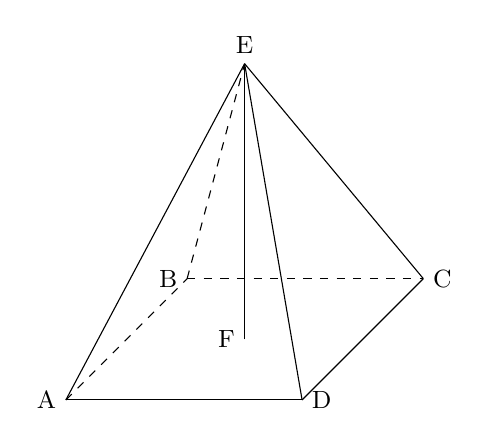
\begin{tikzpicture}[scale=1, transform shape]
    % Define the points of the cube
    \coordinate (A) at (0,0,0);
    \coordinate (B) at (0,0,-4);
    \coordinate (C) at (3,0,-4);
    \coordinate (D) at (3,0,0);
    \coordinate (E) at (1.5,3.5,-2);
    \coordinate (F) at (1.5,0,-2);

    % Draw the visible edges of the cube
    \draw[dashed] (A) -- (B);
    \draw[dashed] (B) -- (C);
    \draw (C) -- (D);
    \draw (A) -- (D);
    
    \draw (A) -- (E);
    \draw (D) -- (E);
    \draw (C) -- (E);
    \draw[dashed] (B) -- (E);

    \draw (F) -- (E);

    % Place the labels with smaller font size
    \node at (A) [left,font=\small] {A};
    \node at (B) [left,font=\small] {B};
    \node at (C) [right,font=\small] {C};
    \node at (D) [right,font=\small] {D};
    \node at (E) [above,font=\small] {E};
    \node at (F) [left,font=\small] {F};
    
\end{tikzpicture}

\begin{tikzpicture}[scale=1, transform shape]
    % Define the points of the cube
    \coordinate (A) at (0,0,0);
    \coordinate (B) at (0,0,-4);
    \coordinate (C) at (3,0,-4);
    \coordinate (D) at (3,0,0);
    \coordinate (E) at (1.5,3.5,-2);

    % Draw the visible edges of the cube
    \draw[dashed] (A) -- (B);
    \draw[dashed] (B) -- (C);
    \draw (C) -- (D);
    \draw (A) -- (D);
    
    \draw (A) -- (E);
    \draw (D) -- (E);
    \draw (C) -- (E);
    \draw[dashed] (B) -- (E);

    % Place the labels with smaller font size
    \node at (A) [left,font=\small] {A};
    \node at (B) [left,font=\small] {B};
    \node at (C) [right,font=\small] {C};
    \node at (D) [right,font=\small] {D};
    \node at (E) [above,font=\small] {E};
\end{tikzpicture}

\end{document}